%loads the class that provides the titlepage and some general packages.
\documentclass{UniVieCS_Thesis} 

%add the additional packages and macros that you want to use
%here you can find some useful additional packages and macros

%Package to show algorithms
\usepackage{algorithm2e}

%package to work with glossaries
\usepackage[acronym]{glossaries}

%packages and setings to show colored code
\usepackage{listings}
\usepackage{xcolor}

\definecolor{codegreen}{rgb}{0,0.6,0}
\definecolor{codegray}{rgb}{0.5,0.5,0.5}
\definecolor{codepurple}{rgb}{0.58,0,0.82}
\definecolor{backcolour}{rgb}{0.95,0.95,0.92}

\lstdefinestyle{mystyle}{
    backgroundcolor=\color{backcolour},   
    commentstyle=\color{codegreen},
    keywordstyle=\color{magenta},
    numberstyle=\tiny\color{codegray},
    stringstyle=\color{codepurple},
    basicstyle=\ttfamily\footnotesize,
    breakatwhitespace=false,         
    breaklines=true,                 
    captionpos=b,                    
    keepspaces=true,                 
    numbers=left,                    
    numbersep=5pt,                  
    showspaces=false,                
    showstringspaces=false,
    showtabs=false,                  
    tabsize=2
}

\lstset{style=mystyle}

%package to allow comments/notes by you and other people
\usepackage[multiuser,marginclue,nomargin,inline,index]{fixme}
\definecolor{ttwgreen}{RGB}{75,135,73}
\fxusetheme{colorsig}
%\FXRegisterAuthor{tm}{atm}{\color{red}TM}
\FXRegisterAuthor{ttw}{attw}{\color{ttwgreen}TTW} % creates ttwnote, ttwwarning, ttwerror, ttwfatal commands
%\FXRegisterAuthor{mk}{amk}{\color{blue}MK}

%add your own packages or macros here

% important update for glossaries, before document 
\loadglsentries{C) Back Matter/acronyms.tex}
\loadglsentries{C) Back Matter/glossary.tex} 
\makeglossaries %https://www.overleaf.com/learn/latex/glossaries

%shows fixme notes
%\fxsetup{status=draft} % comment/delete this line if you want to your final output

\usepackage[ngerman, british]{babel} %if changed to \usepackage[ngerman]{babel} "Table of contents" changes to "Inhaltsverzeichnis", "abstract" becomes "Zusammenfassung" and "references" is translated to "Literatur".


%remove all the things you don't need and add all the things you need. you can also change the order of the elements at your will.
\begin{document}

    %Start with front matter
    
    %Choose the titlepage you want to use
    
    % --CHANGE THE TITLEPAGE HERE

% title page provided in Word by the University which can be found here 
% https://informatik.univie.ac.at/studium/hilfe-fuer-studierende/wegweiser-masterstudium/approbation-der-masterarbeit/ 
% Please pay attention to the guidelines that can be found there!
%


% There are some commands also for multiple lines. If something exceeds more than a line use the multi line commands. In the worst case adjust the vertical spaces within the class.
% -- Title Page
\Title{Characterizing the Fractal Dimension of Molecular Clouds} 
% A title exceeding one line can be created using the \TitleTwo or \TitleThree command
% \TitleTwo{I wish I \\ had a Master's Degree}
% \TitleThree{I wish I \\ had a Master's \\ Degree}
\Who{Simone Spedicato BSc} %Make sure you add all your titles! 
% A name exceeding one line can be created using the \WhoTwo command
% \WhoTwo{ FirstName \\ LastName BSc}
\Degree{Master of Science (MSc)}
\Year{2025}
\ProgrammeCode{066 861}
\ProgrammeName{Master Astronomy} %Make sure it has the same Name as in the Studienblatt
\Supervisor{Assoz. Prof. Dr. Alvaro Hacar Gonzalez, MA}
% \SupervisorTwo{Second Row} % Here you can change the row under the supervisor
\CoSupervisor{0} %remove this line if there is a Co supervisor
% \CoSupervisor{Professor Co}
% \CoSupervisorTwo{Second Row} % Here you can change the row under the cosupervisor

\Titlepage %This generates the titlepage %Creates the titlepage
    %% --CHANGE THE TITLEPAGE HERE

% title page provided in Word by the University which can be found here 
% https://informatik.univie.ac.at/studium/hilfe-fuer-studierende/bachelorarbeit-empfehlungen/ 
% Please pay attention to the guidelines that can be found there!
% If you want you can always create the titlepage in Word and then add it with \includepdf{<filename>} from the pdfpages package to your thesis.
%


%Do not change or delete the following two lines
\renewcommand{\TitleSetup}{BACHELORARBEIT / BACHELOR'S THESIS}
\renewcommand{\TitleTitleSetup}{Titel der Bachelorarbeit / Title of the Bachelor's Thesis\par}
% Change the rest of the lines to fit you thesis

% There are some commands also for multiple lines. If something exceeds more than a line use the multi line commands. In the worst case adjust the vertical spaces within the class.
% -- Title Page
\Title{I wish I had a Bachelor's Degree} 
% A title exceeding one line can be created using the \TitleTwo or \TitleThree command
%\TitleTwo{I wish I \\ had a Bachelor's Degree}
%\TitleThree{I wish I \\ had a Bachelor's \\ Degree}
\Who{ FirstName LastName } %Make sure you add all your titles! 
% A name exceeding one line can be created using the \WhoTwo command
%\WhoTwo{ FirstName \\ LastName }
\Degree{Bachelor of Science (BSc)}
\Year{2019}
\ProgrammeCode{126489}
\ProgrammeName{Masterstudium Informatik} %Make sure it has the same Name as in the Studienblatt
\Supervisor{Univ. Prof. My favorite professor, PhD}
%\SupervisorTwo{Second Row} % Here you can change the row under the supervisor
\CoSupervisor{0} %remove this line if there is a Co supervisor
\CoSupervisor{Professor Co}
\CoSupervisorTwo{Second Row} % Here you can change the row under the cosupervisor

\Titlepage %This generates the titlepage %Creates the titlepage
    %% --CHANGE THE TITLEPAGE HERE

% title page provided in Word by the University which can be found here 
% https://doktorat.univie.ac.at/doktoratsablauf/abschlussphase/einreichen-und-begutachtung/
% Please pay attention to the guidelines that can be found there!
% If you want you can always create the titlepage in Word and then add it with \includepdf{<filename>} from the pdfpages package to your thesis.
%


%Do not change or delete the following two lines
\renewcommand{\TitleSetup}{DISSERTATION / DOCTORAL THESIS}
\renewcommand{\TitleTitleSetup}{Titel der Disseratation / Title of the Doctoral Thesis\par}
% Change the rest of the lines to fit you thesis


% There are some commands also for multiple lines. If something exceeds more than a line use the multi line commands. In the worst case adjust the vertical spaces within the class.
% -- Title Page
\Title{I wish I had a Doctor's Degree} 
% A title exceeding one line can be created using the \TitleTwo or \TitleThree command
%\TitleTwo{I wish I \\ had a Doctor's Degree}
%\TitleThree{I wish I \\ had a Doctor's \\ Degree}
\Who{ FirstName LastName MSc} %Make sure you add all your titles! 
% A name exceeding one line can be created using the \WhoTwo command
%\WhoTwo{ FirstName \\ LastName MSc}
\Degree{Doctor of Philosophy (PhD)}
%\Degree{Doktorin ODER Doktor der >Zusatz< (Dr. >Abkürzung<)}
%\Degree{Doktorin OR Doktor der >affix< (Dr. >abbr.<)}

\Year{2019}
\ProgrammeCode{A 786 880}
\ProgrammeName{Doctoratsstudium Informatik} %Make sure it has the same Name as in the Studienblatt
\Supervisor{Univ. Prof. My favorite professor, PhD}
%\SupervisorTwo{Second Row} % Here you can change the row under the supervisor
\CoSupervisor{0} %remove this line if there is a Co supervisor
\CoSupervisor{Professor Co}
\CoSupervisorTwo{Second Row} % Here you can change the row under the cosupervisor

\Titlepage %This generates the titlepage %Creates the titlepage
    
    \clearpage
	\frontmatter{}
	\thispagestyle{empty}
\chapter{Acknowledgements}

Thank you! 
\clearpage
%\cleardoublepage{} %adds the aknowledgements
			%Please consider the following section of the "Formvorschriften für die gedruckte Version"
	%Im Anhang ist eine Zusammenfassung (Abstract) mitzubinden. 
	%Ist die Arbeit in einer Fremdsprache verfasst, ist im Anhang jedenfalls eine deutsche Zusammenfassung mitzubinden.
\chapter{Abstract}
		This \LaTeX{} template provides example on how to format and display text, 
		mathematical formulas, and insert tables or images. There is a lot more you 
		can do with \LaTeX{}, for more information check out https://en.wikibooks.org/wiki/LaTeX.
 % adds the abstract
	\chapter{Kurzfassung}

Die Struktur von Molekülwolken ist entscheidend für das Verständnis der physikalischen Prozesse, die die Sternentstehung steuern. In dieser Arbeit präsentieren wir eine detaillierte morphologische und topologische Analyse der Molekülwolken Orion~A und Orion~B mithilfe von Methoden der Fraktalgeometrie und Minkowski-Funktionale. Auf Basis von Säulendichtekarten, die aus Staubemissionen im fernen Infrarot gewonnen wurden, bestimmen wir sowohl globale als auch lokale fraktale Dimensionen über einen breiten Dynamikbereich hinweg.

Unsere Ergebnisse zeigen in Orion~A einen strukturellen Übergang bei einer Säulendichte von $N \sim 1{,}2 \times 10^{22} \,\mathrm{cm}^{-2}$, der mit dem Auftreten dichter Kerne und erhöhter Sternentstehungsaktivität zusammenfällt. Orion~B hingegen weist eine durchgängig skalenfreie, turbulente Morphologie ohne einen solchen Übergang auf. Die Euler-Charakteristik untermauert diese Interpretation durch ein deutliches topologisches Maximum in Orion~A, das in Orion~B fehlt. 

Zusätzlich führen wir eine lokale Karte der fraktalen Dimension sowie sogenannte Masse–Größe–Dimensions–Diagramme (MSD) ein, um die strukturelle Komplexität ortsaufgelöst zu analysieren. Ein Vergleich mit der Verteilung junger Sternobjekte (YSOs) zeigt, dass Regionen mit höherer fraktaler Komplexität insbesondere in Orion~A vermehrt frühe Entwicklungsstadien der Sternentstehung aufweisen. Dies deutet auf eine Verbindung zwischen komplexer Morphologie und aktiver Sternbildung hin.

Unsere Arbeit zeigt, wie Methoden der Fraktal- und Topologieanalyse helfen können, die mehrskalige Struktur des interstellaren Mediums zu erfassen und mit physikalischen Prozessen der Sternentstehung zu verknüpfen.

\clearpage %adds the "Kurzfassung"in german.
	\pagebreak
	
    \microtypesetup{protrusion=false}
    \tableofcontents{}
    % Use an optional list of tables / figures / algorithms / listings(code).
    \listoftables 
    \listoffigures
    \cleardoublepage{}
    \listofalgorithms
    \addcontentsline{toc}{chapter}{List of Algorithms} 
    \cleardoublepage{}
    \lstlistoflistings
    \cleardoublepage{}
    \microtypesetup{protrusion=true}
    
	\pagebreak
	
	%add your chapters here
	\mainmatter{}
    \chapter{Using the template}
	
Welcome to the Latex Template of the Computer Science department of the university of Vienna. 
\url{https://informatik.univie.ac.at/en/}

General information about finishing your Bachelors degree can be found here:
\begin{enumerate}
    \item \url{https://informatik.univie.ac.at/studium/hilfe-fuer-studierende/studienabschluss/abschluss-des-bachelor-studiums/}
    \item \url{https://informatik.univie.ac.at/studium/hilfe-fuer-studierende/bachelorarbeit-empfehlungen/}
\end{enumerate}

General information about finishing your Masters degree can be found here:
\begin{enumerate}
    \item \url{https://informatik.univie.ac.at/studium/hilfe-fuer-studierende/wegweiser-masterstudium/approbation-der-masterarbeit/}
    \item \url{https://informatik.univie.ac.at/studium/hilfe-fuer-studierende/wegweiser-masterstudium/anmeldung-masterarbeit-themenfindung/}
    \item \url{https://informatik.univie.ac.at/studium/hilfe-fuer-studierende/wegweiser-masterstudium/anmeldung-zur-masterpruefung/}
\end{enumerate}

General information about finishing your Doctors degree can be found here:
\begin{enumerate}
    \item \url{https://doktorat.univie.ac.at/doktoratsablauf/abschlussphase/einreichen-und-begutachtung/}

\end{enumerate}
	
\section{Using the template}

Everything in the template revolves around the \verb|main.tex| file. Here all the other files are put together to create the thesis.
There are 3 different sections to consider: Front Matter, Chapters and Back Matter. Each section has a folder where you can put the different parts of your thesis. In the Front Matter section you should put everything that comes before your first chapter of the thesis. Respectively, in the Back Matter section you put everything that comes after your last chapter. And finally all the chapters are put into the Chapters folder. You can put thing like abstract, summaries, etc... wherever they suit your thesis. In the end it really only matters how you add them into your \verb|main.tex| file. With the \verb|\input{}| command you can add the parts if they should appear in your thesis, the order within the \verb|main.tex| also determines the order in the final pdf. Also depending on whether you do your BSc, MSc or Phd you should add the corresponding titlepage in the main.tex file and then delete the tex files of the other two.

\subsection{Title-page}
The Layout of the Title-page is in the \verb|UniVieCS_Thesis.cls| and should normally not be changed. You can use all the commands as seen in the \verb|Titlepage.tex|. 

The template and also the title-page is based on the scrbook class. So if you want to use a different class without changing the title page I would recommend using the template for creating the title page and then use it in your project using the 
\verb|\includepdf{<filename>}| from the \verb|pdfpages| package. \textbf{Alternatively, if you encounter any problems with the title page, you can also always use the word template for the title- page and add it using this package.} In that way you can avoid any differences to the original title page template. The word templates can be found here:
\begin{enumerate}
    \item \url{https://informatik.univie.ac.at/en/study/support-for-students/bachelor-thesis-guidelines/}
    \item \url{https://informatik.univie.ac.at/studium/hilfe-fuer-studierende/wegweiser-masterstudium/approbation-der-masterarbeit/ }
    \item \url{https://doktorat.univie.ac.at/doktoratsablauf/abschlussphase/einreichen-und-begutachtung/}

\end{enumerate}

If you use the \verb|includepdf| package make sure that the pdf still has the correct metadata afterwards.


\section{Creating the pdf}
To create a proper pdf file of your thesis there are some things to consider
\subsection{Embed all fonts in pdf}
Please make sure that you embed all fonts in your pdf. Also make sure all the fonts of any figures that were used in the document are embedded. 
If you don't use any pdf figures pdfLaTeX should embed all fonts automatically.

\subsubsection{Linux}
On Linux you can use the command \begin{verbatim}
    pdffonts my_file.pdf
\end{verbatim}
to check if the fonts are embbeded. Check if all the fonts listed have a "yes" in the "emb" column. 
\begin{verbatim}
name                                 type              encoding         emb sub uni 
------------------------------------ ----------------- ---------------- --- --- --- 
BXJBCJ+NimbusSanL-Bold               Type 1            Custom           yes yes no     
HEMYJL+NimbusSanL-Regu               Type 1            Custom           yes yes no     
OOJWDR+SFRM1000                      Type 1            Custom           yes yes no      
OHLNOC+SFRM0900                      Type 1            Custom           yes yes no   
...
\end{verbatim}
For more information see 

\url{https://www.karlrupp.net/2016/01/embed-all-fonts-in-pdfs-latex-pdflatex/}
\subsubsection{Windows}
On Windows using the Adobe Acrobat Reader the fonts can be found at
\begin{verbatim}
File > Properties > Fonts
\end{verbatim}
For more information please consult
\begin{enumerate}
\item \url{https://helpx.adobe.com/acrobat/using/pdf-fonts.html}

\item \url{https://www.overleaf.com/learn/latex/Questions/My_submission_was_rejected_by_the_journal_because_%22Font_XYZ_is_not_embedded%22._What_can_I_do%3F} 
\end{enumerate}

\subsection{Making a PDF/A-1 compatible pdf}
% Making the the work PDF/A compatible:
%"Für die Ablieferung Ihrer Abschlussarbeit in elektronischer Form sind als einziges Dateiformat PDF-Dokumente in der von Adobe spezifizierten Version PDF/A-1 bzw. PDF/A-2 erlaubt."
% https://hopla.univie.ac.at/erstellen_von_pdf.pdf
As can be seen in \url{https://hopla.univie.ac.at/erstellen_von_pdf.pdf} and the "Informationen zur Erstellung und Abgabe von Hochschulschriften" it is required to provide a PDF/A-1 or PDF/A-2 version of your thesis.

\subsubsection{validation}
To validate the produced PDF you can either use the Preflight tool included in Adobe Acrobat Pro or a free online version. E.g. \url{https://www.pdf-online.com/osa/validate.aspx}.
Please take caution as different validation tools can report different results.

\subsubsection{pdfx}
First step to get PDF/A combatibility is by using the package \verb|pdfx| - make sure it is included before the hyperref package.
\begin{verbatim}
\usepackage[a-1b]{pdfx}
\end{verbatim}
This package is already included in the class.
For more details about the package and the following steps please consult \url{http://texdoc.net/texmf-dist/doc/latex/pdfx/pdfx.pdf}

\subsubsection{metadata}
There is a section in the beginning of the .tex file where you can change the metadata.
Change your Name, Title, Subject, Keywords and remove/add Information as you like. To find out what fields are possible please check here. \url{http://texdoc.net/texmf-dist/doc/latex/pdfx/pdfx.pdf#subsection.2.3}

A file containing the metadata (jobname.xmpdata) is created when compiling. 

Watch out, the metadata .xmpdata file is only created one time. So if you need to update it you need to clear the cache of overleaf. Or delete the .xmpdata file. It is then recreated the next time you compile. 

\url{https://www.overleaf.com/learn/how-to/Clearing_the_cache}

You can check the metadata of your PDF with Acrobat Reader by going to File-> properties. Or alternatively check it with an online tool.

\subsubsection{figures}
As already mentioned, make sure that all the fonts used in the pictures are included. Furthermore transparency in pictures causes issues, please convert transparent figures into their nontransparent version. 

Using Linux the command \verb|pdfimages -list <pdf>| shows the typpe of all images used. The type should always be \verb|image| and not \verb|smask|. Check and convert these images.

\subsubsection{color}
Additionally there can be problems if figures use different color spaces. Use the same command as before and check if all images use the same color. 

If color is really important in your work it might also be a good idea to use an ICC profile for the color. 
For more details about colors check \url{http://texdoc.net/texmf-dist/doc/latex/pdfx/pdfx.pdf#subsection.2.5}

It is also possible to convert the pictures automatically using ghostscript. But always check the results manually. 

\subsubsection{Other errors}
Due to the complexity of Latex files there can be many more errors that are not covered in the readme.

The Preflight tool included in Adobe Acrobat Pro also has the ability to fix some errors. For example EOL (End of Line) errors can be fixed with its analyize and fix option. 
Please also check if any of the following pages might have a solution to your problem:
\begin{enumerate}
    \item \url{https://www.mathstat.dal.ca/~selinger/pdfa/}
    \item \url{https://blog.zhaw.ch/icclab/creating-pdfa-documents-for-long-term-archiving/}
    \item german: \url{http://kulturreste.blogspot.com/2014/06/grrrr-oder-wie-man-mit-latex-vielleicht.html}
    \item \url{https://support.stmdocs.in/wiki/?title=Generating_PDF/A_compliant_PDFs_from_pdftex}
    \item \url{http://texdoc.net/texmf-dist/doc/latex/pdfx/pdfx.pdf}
\end{enumerate}

\subsubsection{Tagged PDF}
Currently with Latex it is only possible to create files that are in the PDF/A-1b format. The PDF/A-1a format required the PDF to be tagged which is currently not possible in a satisfactory way.
A manual tagging with Adobe Acrobat Pro is possible but not recommended.

More information about the current status of tagged pdfs can be found here:
\begin{enumerate}
\item \url{https://umij.wordpress.com/2016/08/11/the-sad-state-of-pdf-accessibility-of-latex-documents/} 
\item \url{https://www.tug.org/TUGboat/tb30-2/tb95moore.pdf}
\end{enumerate}

\subsection{General Remarks to create the pdf}
Highest priority should always be the embedding of all fonts. Further compliance with the PDF/A standards is always desired, but talk to your supervisor in any case.

Please also check the following resources if you have problems and need assistance

\begin{enumerate}
\item \url{https://spl29.univie.ac.at/fileadmin/user_upload/s_spl29/Studium/abschluss_master/Infoblatt_Hochschulschriften.pdf} 
\item \url{https://e-theses.univie.ac.at/E-Theses_erstellen_von_pdf.pdf}
\end{enumerate}

\section{Further tips on the template}
In the following chapters there are some general tips on the elements of Latex. You can check them out if you think they have useful information for you. Then you delete these chapters and replace them with the real chapters of your thesis.

Also don't forget to register your Thesis at:
\url{https://informatik.univie.ac.at/studium/hilfe-fuer-studierende/wegweiser-masterstudium/anmeldung-masterarbeit-themenfindung/}

    	\chapter{Ordinary Text} 	% Produces section heading.  Lower-level
	
    % A '%' character causes TeX to ignore all remaining text on the line,
    % and is used for comments like this one.

	% sections are begun with similar 
	% \subsection and \subsubsection commands.
	
	The ends  of words and sentences are marked 
	by   spaces. It  doesn't matter how many 
	spaces    you type; one is as good as 100.  The
	end of   a line counts as a space.
	
	One   or more   blank lines denote the  end 
	of  a paragraph.  
	
	Since any number of consecutive spaces are treated
	like a single one, the formatting of the input
	file makes no difference to
	\LaTeX,                % The \LaTeX command generates the LaTeX logo.
	but it makes a difference to you.  When you use 
	\LaTeX \cite{lamport94},  % \cite inserts a reference, which you define at the end of the document
	making your input file as easy to read
	as possible will be a great help as you write 
	your document and when you change it.  This sample 
	file shows how you can add comments to your own input 
	file.
	
	Because printing is different from typewriting,
	there are a number of things that you have to do
	differently when preparing an input file than if
	you were just typing the document directly.
	Quotation marks like
	``this'' 
	have to be handled specially, as do quotes within
	quotes:
	``\,`this'            % \, separates the double and single quote.
	is what I just 
	wrote, not  `that'\,''.  
	
	Dashes come in three sizes: an 
	intra-word 
	dash, a medium dash for number ranges like 
	1--2, 
	and a punctuation 
	dash---like 
	this.
	
	A sentence-ending space should be larger than the
	space between words within a sentence.  You
	sometimes have to type special commands in
	conjunction with punctuation characters to get
	this right, as in the following sentence.
	Gnats, gnus, etc.\ all  % `\ ' makes an inter-word space.
	begin with G\@.         % \@ marks end-of-sentence punctuation.
	You should check the spaces after periods when
	reading your output to make sure you haven't
	forgotten any special cases.  Generating an
	ellipsis
	\ldots\               % `\ ' is needed after `\ldots' because TeX 
	% ignores spaces after command names like \ldots 
	% made from \ + letters.
	%
	% Note how a `%' character causes TeX to ignore 
	% the end of the input line, so these blank lines 
	% do not start a new paragraph.
	%
	with the right spacing around the periods requires
	a special command.
	
	\LaTeX\ interprets some common characters as
	commands, so you must type special commands to
	generate them.  These characters include the
	following:
	\$ \& \% \# \{ and \}.
	
	In printing, text is usually emphasized with an
	\emph{italic}  
	type style.  
	
	\begin{em}
		A long segment of text can also be emphasized 
		in this way.  Text within such a segment can be 
		given \emph{additional} emphasis.
	\end{em}
	
	It is sometimes necessary to prevent \LaTeX\ from
	breaking a line where it might otherwise do so.
	This may be at a space, as between the ``Mr.''\ and
	``Jones'' in
	``Mr.~Jones'',        % ~ produces an unbreakable interword space.
	or within a word---especially when the word is a
	symbol like
	\mbox{\emph{itemnum}} 
	that makes little sense when hyphenated across
	lines.
	
	Footnotes\footnote{This is an example of a footnote.}
	pose no problem.
	
	\LaTeX\ is good at typesetting mathematical formulas
	like
	\( x-3y + z = 7 \) 
	or
	\( a_{1} > x^{2n} + y^{2n} > x' \)
	or  
	\( AB  = \sum_{i} a_{i} b_{i} \).
	The spaces you type in a formula are 
	ignored.  Remember that a letter like
	$x$                   % $ ... $  and  \( ... \)  are equivalent
	is a formula when it denotes a mathematical
	symbol, and it should be typed as one.
	Furthermore you can add a formula as Images or Tables, see Formula  \hyperref[eq:abc]{\ref{eq:abc}}
	\begin{equation}
	\label{eq:abc}
	a+b=c
	\end{equation}
	
		It is sometimes necessary to prevent \LaTeX\ from
	breaking a line where it might otherwise do so.
	This may be at a space, as between the ``Mr.''\ and
	``Jones'' in
	``Mr.~Jones'',        % ~ produces an unbreakable interword space.
	or within a word---especially when the word is a
	symbol like
	\mbox{\emph{itemnum}} 
	that makes little sense when hyphenated across
	lines.
    	\chapter{Displayed Text}
	
	Text is displayed by indenting it from the left
	margin.  Quotations are commonly displayed.  There
	are short quotations
	\begin{quote}
		This is a short quotation.  It consists of a 
		single paragraph of text.  See how it is formatted.
	\end{quote}
	and longer ones.
	\begin{quotation}
		This is a longer quotation.  It consists of two
		paragraphs of text, neither of which are
		particularly interesting.
		
		This is the second paragraph of the quotation.  It
		is just as dull as the first paragraph.
	\end{quotation}
	Another frequently-displayed structure is a list.
	The following is an example of an \emph{itemized}
	list.
	\begin{itemize}
		\item This is the first item of an itemized list.
		Each item in the list is marked with a ``tick''.
		You don't have to worry about what kind of tick
		mark is used.
		
		\item This is the second item of the list.  It
		contains another list nested inside it.  The inner
		list is an \emph{enumerated} list.
		\begin{enumerate}
			\item This is the first item of an enumerated 
			list that is nested within the itemized list.
			
			\item This is the second item of the inner list.  
			\LaTeX\ allows you to nest lists deeper than 
			you really should.
		\end{enumerate}
		This is the rest of the second item of the outer
		list.  It is no more interesting than any other
		part of the item.
		\item This is the third item of the list.
	\end{itemize}
	You can even display poetry.
	\begin{verse}
		There is an environment 
		for verse \\             % The \\ command separates lines
		Whose features some poets % within a stanza.
		will curse.   
		
		% One or more blank lines separate stanzas.
		
		For instead of making\\
		Them do \emph{all} line breaking, \\
		It allows them to put too many words on a line when they'd rather be 
		forced to be terse.
	\end{verse}
	
	Mathematical formulas may also be displayed.  A
	displayed formula 
	is 
	one-line long; multiline
	formulas require special formatting instructions.
	\[  \Gamma \times  \psi = x'' + y^{2} + z_{i}^{n}\]
	Don't start a paragraph with a displayed equation,
	nor make one a paragraph by itself.
    	\chapter{Tables and Images}
	One of the great advantages of \LaTeX{} is that all it needs to know is
	the structure of a document, and then it will take care of the layout
	and presentation itself.  So, here we shall begin looking at how exactly
	you tell \LaTeX{} what it needs to know about your document.
	
	\subsection{Tables}
	In this sub-section, a simple table is inserted. To add reference to the table, see (cf. Table~\hyperref[tab:table example]{\ref{tab:table example}}):
	
	%A simple table.  The center environment is first set up, otherwise the
	%table is left aligned.  The tabular environment is what tells Latex
	%that the data within is data for the table.
	\begin{table}[htb]
		\centering
		\begin{tabular}{|p{5,5cm}|c|}
			%The tabular environment is what tells Latex that the data within is
			%data for the table.  The arguments say that there will be two
			%columns, both left justified (indicated by the 'l', you could also
			%have 'c' or 'r'.  The bars '|' indicate vertical lines throughout
			%the table.
			
			\hline  % Print horizontal line
			Command & Level \\ \hline  % Columns are delimited by '&'.  And
			%rows are delimited by '\\'
			\texttt{\textbackslash part\{\emph{part}\}} & -1 \\
			\texttt{\textbackslash chapter\{\emph{chapter}\}} & 0 \\
			\texttt{\textbackslash section\{\emph{section}\}} & 1 \\
			\texttt{\textbackslash subsection\{\emph{subsection}\}} & 2 \\
			\texttt{\textbackslash subsubsection\{\emph{subsubsection}\}} & 3 \\
			\texttt{\textbackslash paragraph\{\emph{paragraph}\}} & 4 \\
			\texttt{\textbackslash subparagraph\{\emph{subparagraph}\}} & 5 \\
			\hline
			
		\end{tabular}
		\caption{some description of the table}
		\label{tab:table example}
	\end{table}
	
	\subsection{Images}
	% Here is how to insert an image as a figure. There is a lot more you can do
	% when inserting images, check out: https://en.wikibooks.org/wiki/LaTeX/Importing_Graphics
	
	\begin{figure}[ht]
		\centering
		
\includegraphics[width=0.3\textwidth]{figures/logo_nontransparent.jpg}
		\caption{Image Example}
		\label{fig:image_example}
	\end{figure}
	
	When an image is inserted, you can refer to it like this (cf. Figure~\hyperref[fig:image_example]{\ref{fig:image_example}}).
	
	\subsubsection{A Subsubsection}
	As one last example, this is how you can insert a sub-sub-section! Have fun
	writing your thesis with \LaTeX{}!
	
	\pagebreak
    \chapter{Code}
If you want to show program code within your thesis you can use the \verb|\texttt{verbatim}| environment or for a more complex display take a look at \url{https://www.overleaf.com/learn/latex/Code_listing}

\begin{verbatim}
Text enclosed inside \texttt{verbatim} environment 
is printed directly 
and all \LaTeX{} commands are ignored.
\end{verbatim}

\begin{lstlisting}[language=Python, caption=Python example]
import numpy as np
    
def incmatrix(genl1,genl2):
    m = len(genl1)
    n = len(genl2)
    M = None #to become the incidence matrix
    VT = np.zeros((n*m,1), int)  #dummy variable
    
    #compute the bitwise xor matrix
    M1 = bitxormatrix(genl1)
    M2 = np.triu(bitxormatrix(genl2),1) 

    for i in range(m-1):
        for j in range(i+1, m):
            [r,c] = np.where(M2 == M1[i,j])
            for k in range(len(r)):
                VT[(i)*n + r[k]] = 1;
                VT[(i)*n + c[k]] = 1;
                VT[(j)*n + r[k]] = 1;
                VT[(j)*n + c[k]] = 1;
                
                if M is None:
                    M = np.copy(VT)
                else:
                    M = np.concatenate((M, VT), 1)
                
                VT = np.zeros((n*m,1), int)
    
    return M
\end{lstlisting}
    

\chapter{Algorithms}

If you want to show algorithms in your Thesis take a look at the \url{https://www.overleaf.com/learn/latex/algorithms} page. The \verb|algorithm2e| package is already included in the template. You can list algorithms in the same way as you can list Tables and Figures.

\begin{algorithm}[H]
 \KwData{this text}
 \KwResult{how to write algorithm with \LaTeX2e }
 initialization\;
 \While{not at end of this document}{
  read current\;
  \eIf{understand}{
   go to next section\;
   current section becomes this one\;
   }{
   go back to the beginning of current section\;
  }
 }
 \caption{How to write algorithms}
\end{algorithm}
\cleardoublepage{}

    \chapter{Acronyms and Glossary.}

if you want to use Acronyms or a Glossary check the page here: \url{https://www.overleaf.com/learn/latex/glossaries}

The \Gls{latex} typesetting markup language is specially suitable 
for documents that include \gls{maths}. are 
rendered properly an easily once one gets used to the commands.

Given a set of numbers, there are elementary methods to compute 
its \acrlong{gcd}, which is abbreviated \acrshort{gcd}. This 
process is similar to that used for the \acrfull{lcm}.
    \chapter{Macros}

You can also add useful packages or macros into the \verb|packages_macros.tex| file to add them to the project.
The packages for algorithms, code or the glossary have already been added there.

\subsubsection{FixMe}
Another example, the \verb|FixMe| package, is added as well. It allows you or your supervisor to add Meta comments to the document. These comments only appear if you set the draft mode in the \verb|main.tex| file. If you remove or comment the activation of the draft mode you can see your final thesis without comments. 
%to see the final output comment the line \fxsetup{status=draft} in the main.tex
\fxnote[inline]{This line can only be seen if the draft mode is set in the main.tex}
    
	%add your sources in the bib file and change the style here
    \bibliographystyle{alpha}
	\bibliography{bibliography}
	
	\printglossary[type=\acronymtype]
    \printglossary

    \cleardoublepage{}
	\pagebreak
	
	%add your end matter here
	\appendix{}

	\chapter{Appendix}

This first appendix contains extra graphs and results that mainly compliment the results section. 
\section{Fractal Dimension}
% Dendrograms (maybe)

This section shows more plots regarding the local fractal dimension and the evolution of structures on the Mass-Size-Fractal Dimension graph.
% to-do
% likely to redo, very messy
\begin{figure}[h]
    \centering
    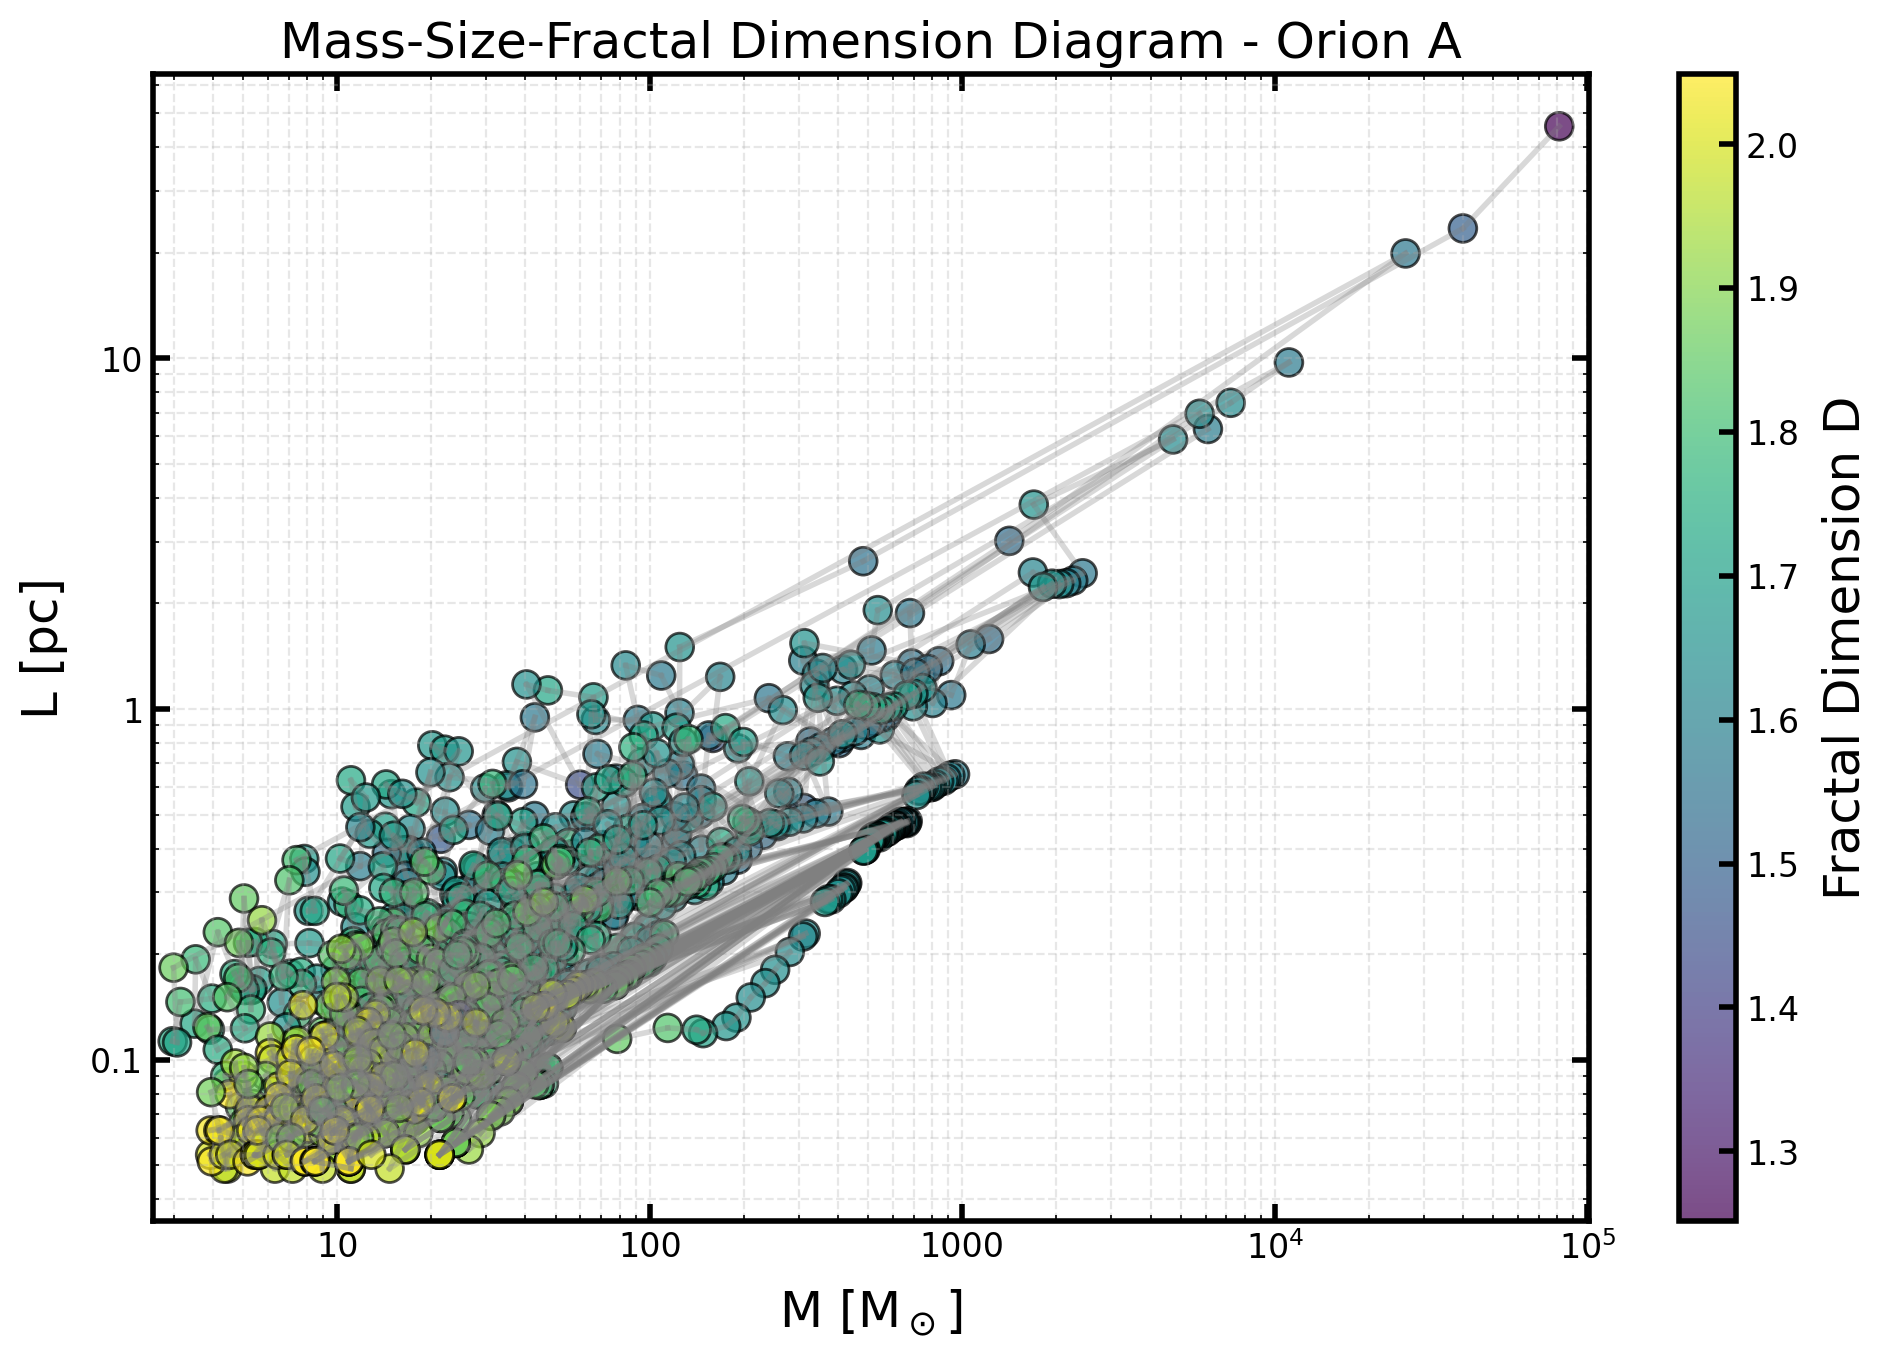
\includegraphics[width=0.5\textwidth]{figures/MSD_Orion_A_with_lines.png}
    \caption{MSD plane for Orion~A with dendrogram connections overplotted. Lines trace parent-child relationships between structures.}
    \label{fig:MSD_orion_A_lines}
\end{figure}

\begin{figure}[h]
    \centering
    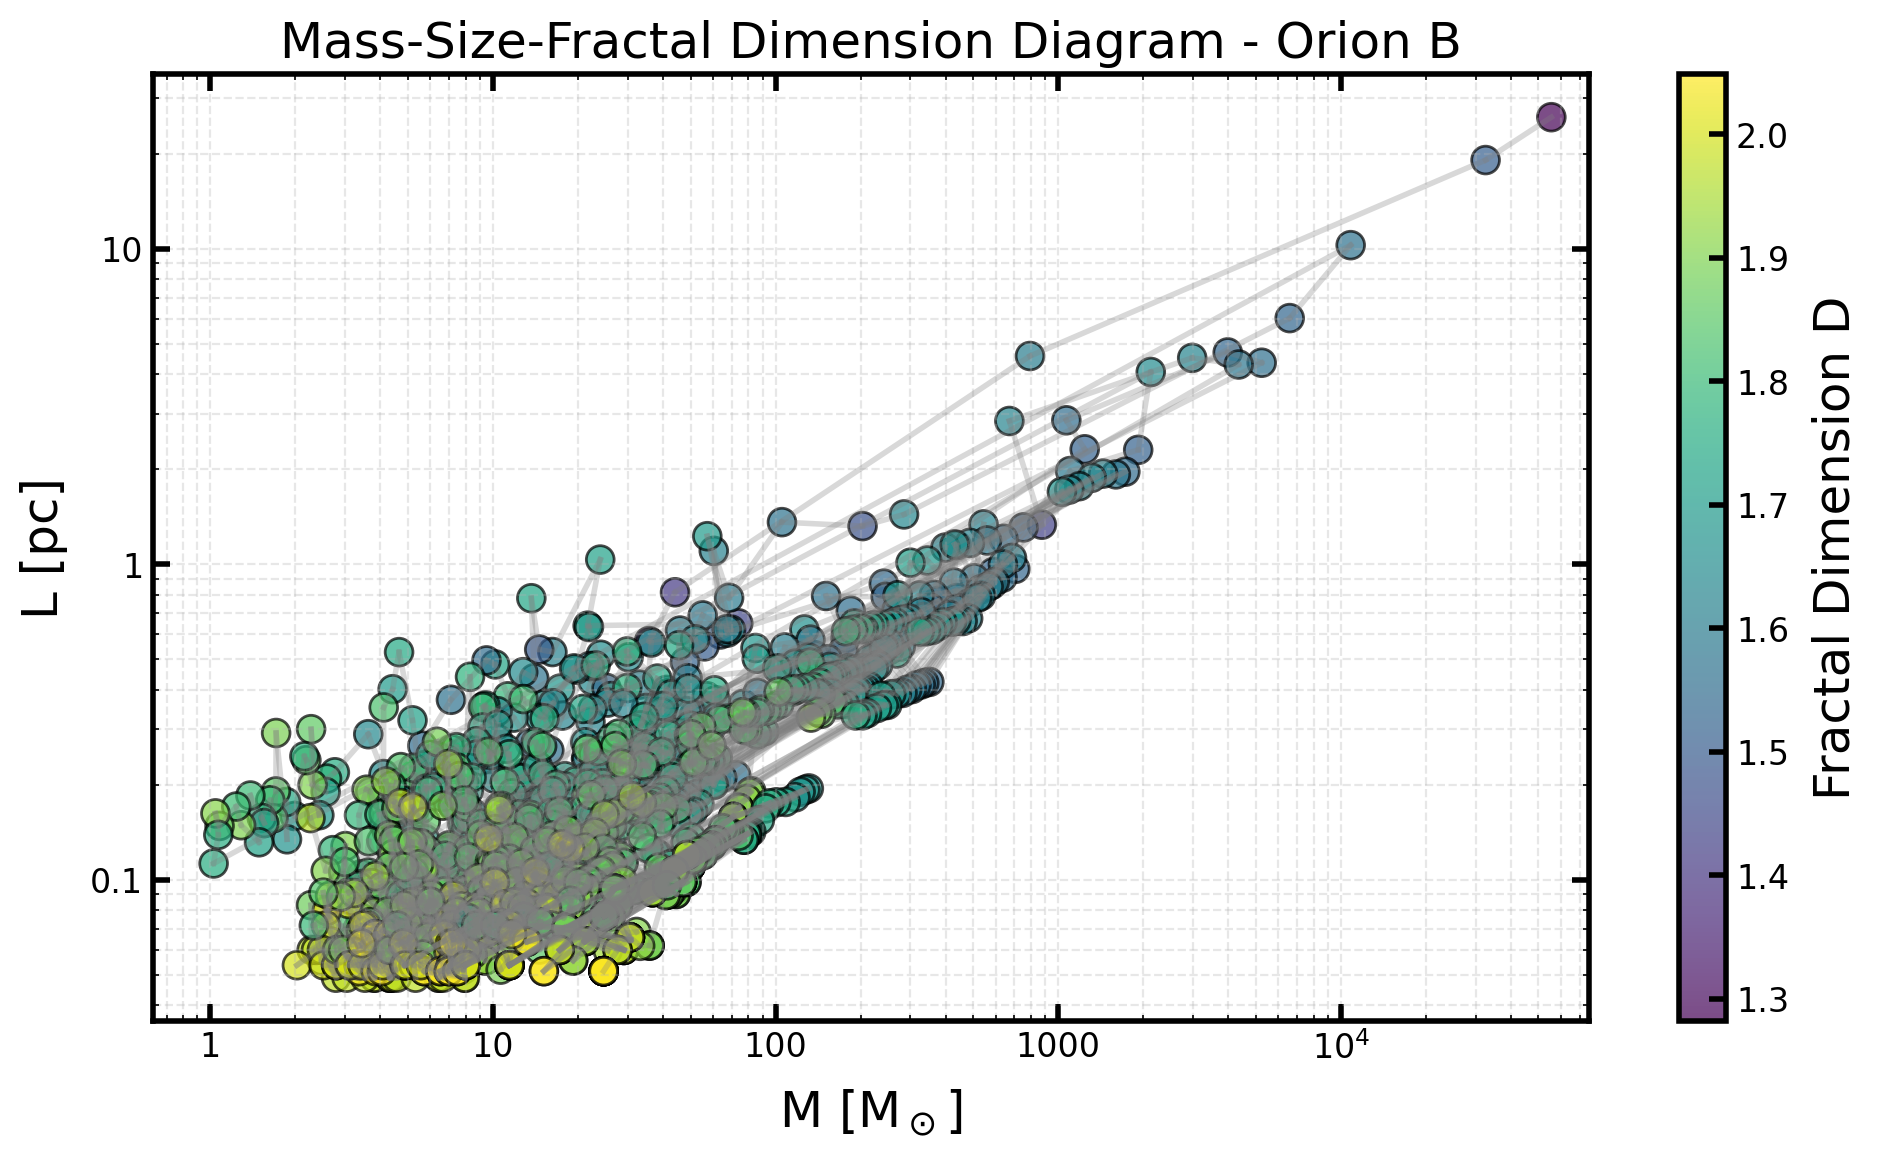
\includegraphics[width=0.5\textwidth]{figures/MSD_Orion_B_with_lines.png}
    \caption{MSD plane for Orion~B with dendrogram connections overplotted.}
    \label{fig:MSD_orion_B_lines}
\end{figure}

\section{YSO Density Maps}

This section of the appendix provides the YSO density maps used in the correlation analysis discussed in the main text.  

\subsection{Class I/flat-spectrum sources}

The following maps show the surface density of early‑stage YSOs (Class~I and flat‑spectrum) for Orion~A and Orion~B.  
These objects are most closely associated with ongoing star formation and are used in the analysis to trace regions of active star‑forming activity.

\begin{figure}[h]
    \centering
    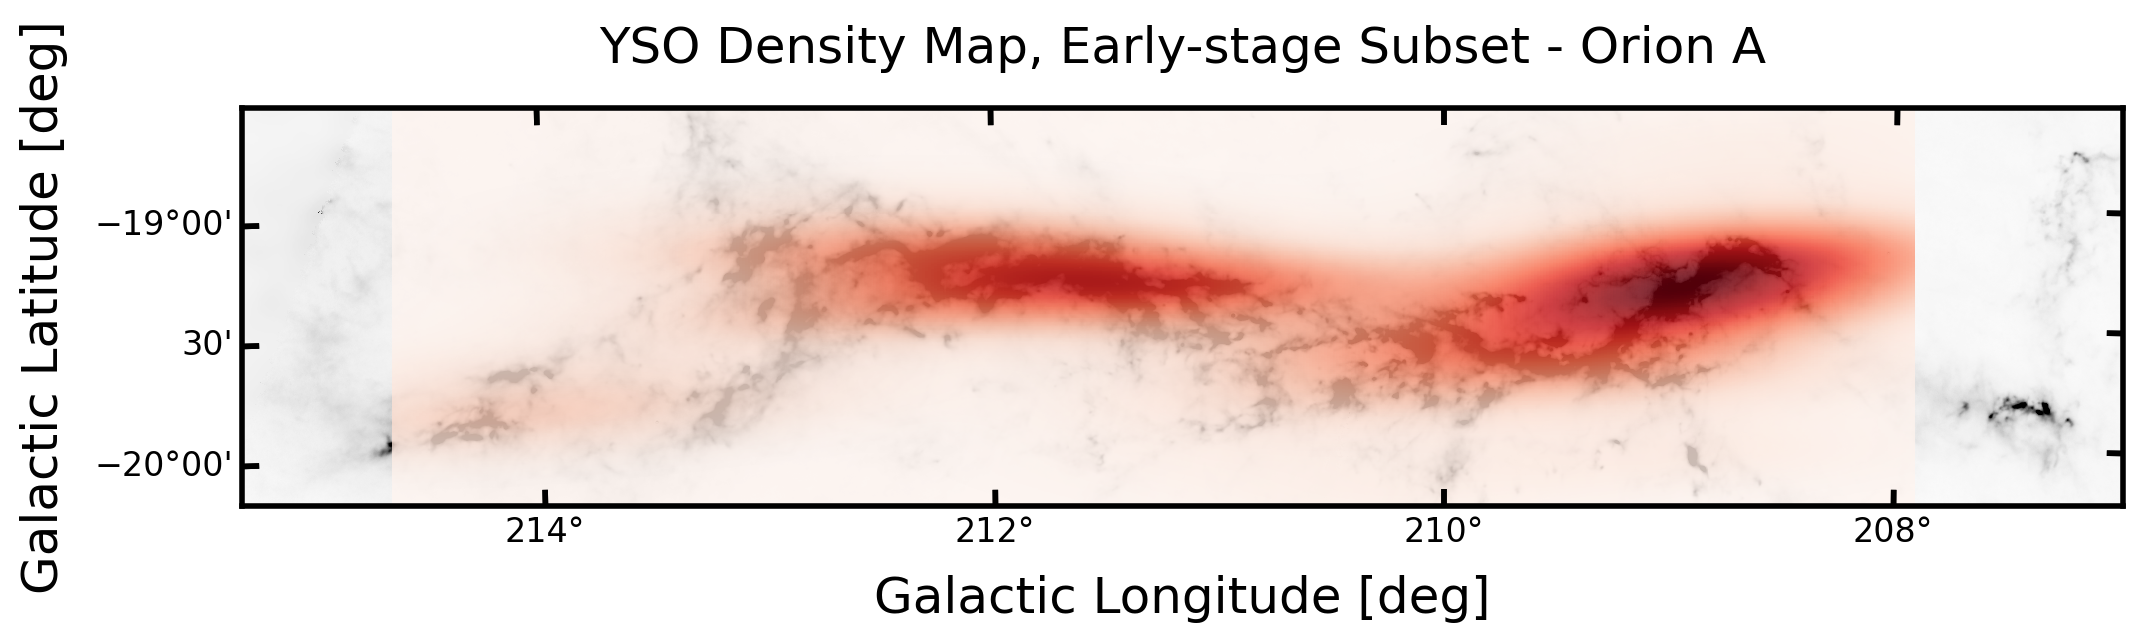
\includegraphics[width=0.75\textwidth]{figures/YSOs_early_stage_density_Orion_A.png}
    \caption{YSO density map for Orion~A, overlaid on the column-density map. The coverage is limited by the extent of the YSO catalog, so some regions are not sampled.}
    \label{fig:YSOs_density_Map_A_early_stages}
\end{figure}

\begin{figure}[h]
    \centering
    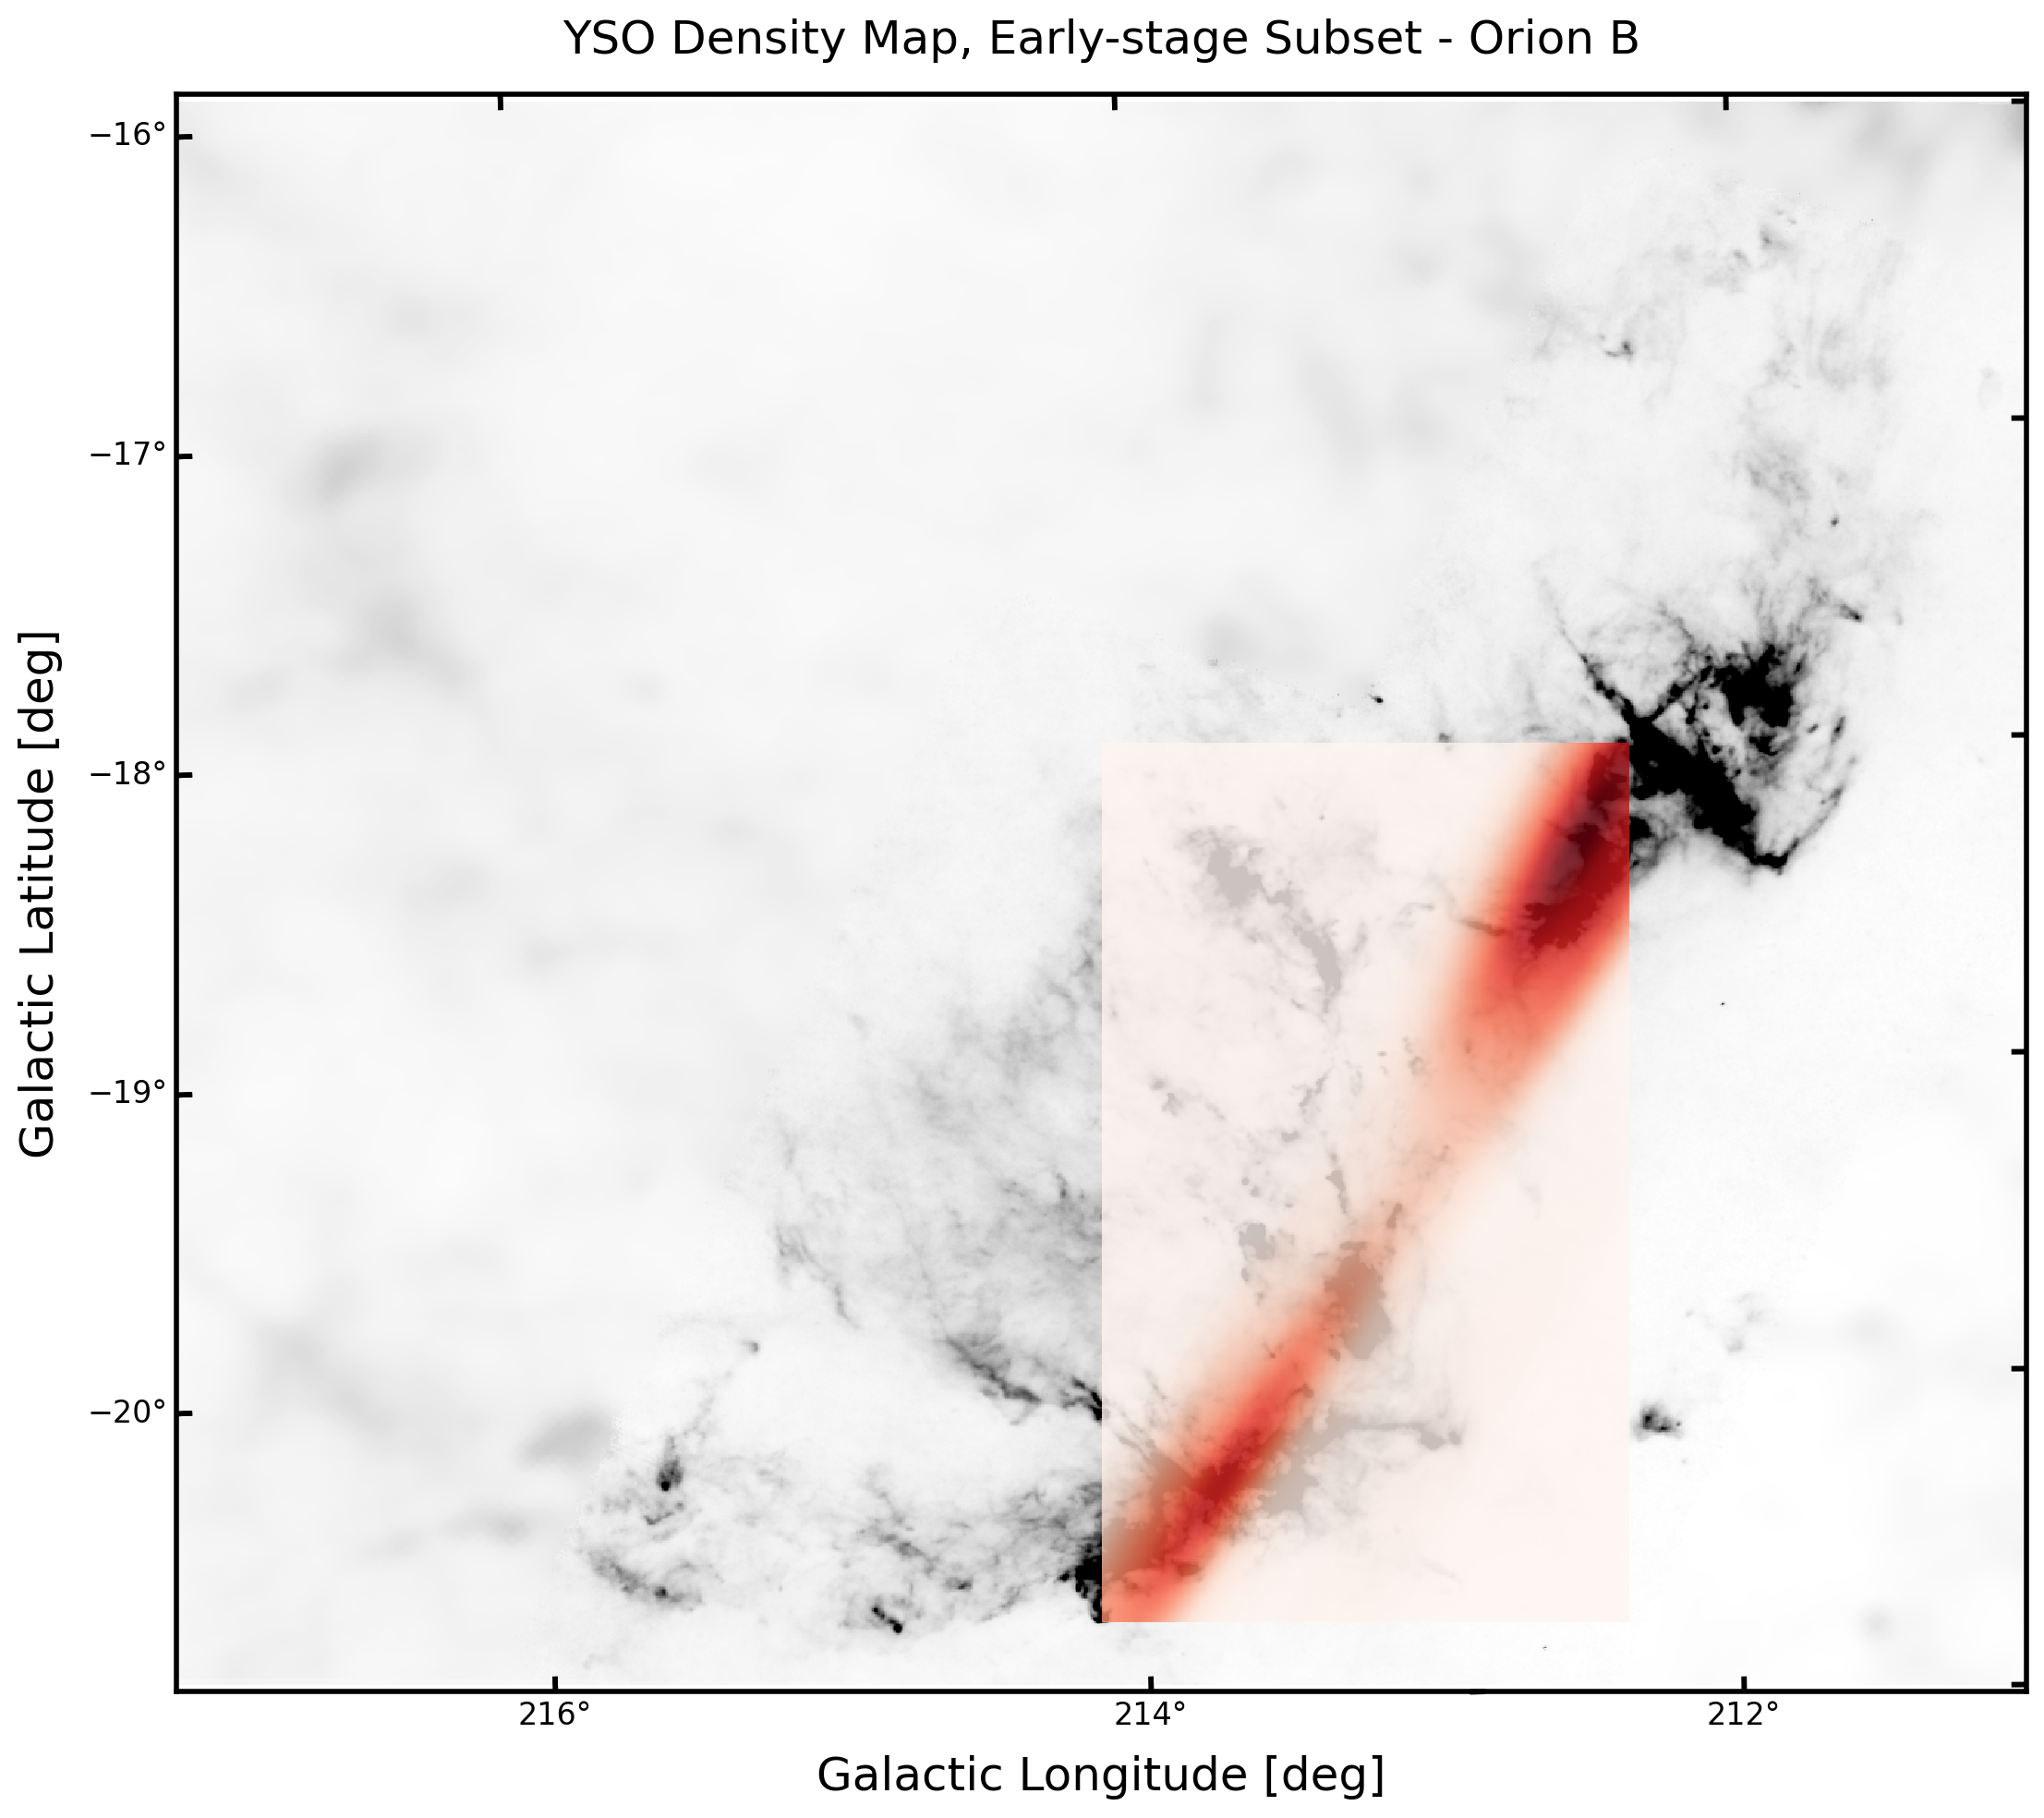
\includegraphics[width=0.5\textwidth]{figures/YSOs_early_stage_density_Orion_B.png}
    \caption{YSO density map for Orion~A, overlaid on the column-density map. The coverage is limited by the extent of the YSO catalog, so some regions are not sampled.}
    \label{fig:YSOs_density_Map_B_early_stages}
\end{figure}

\subsection{Full Sample}

The next set of maps shows the surface density for the full YSO sample, including more evolved Class~II sources.  
These maps provide a broader view of the stellar content but include stars that may have migrated from their birth sites, resulting in a more diffuse distribution.

\begin{figure}[h]
    \centering
    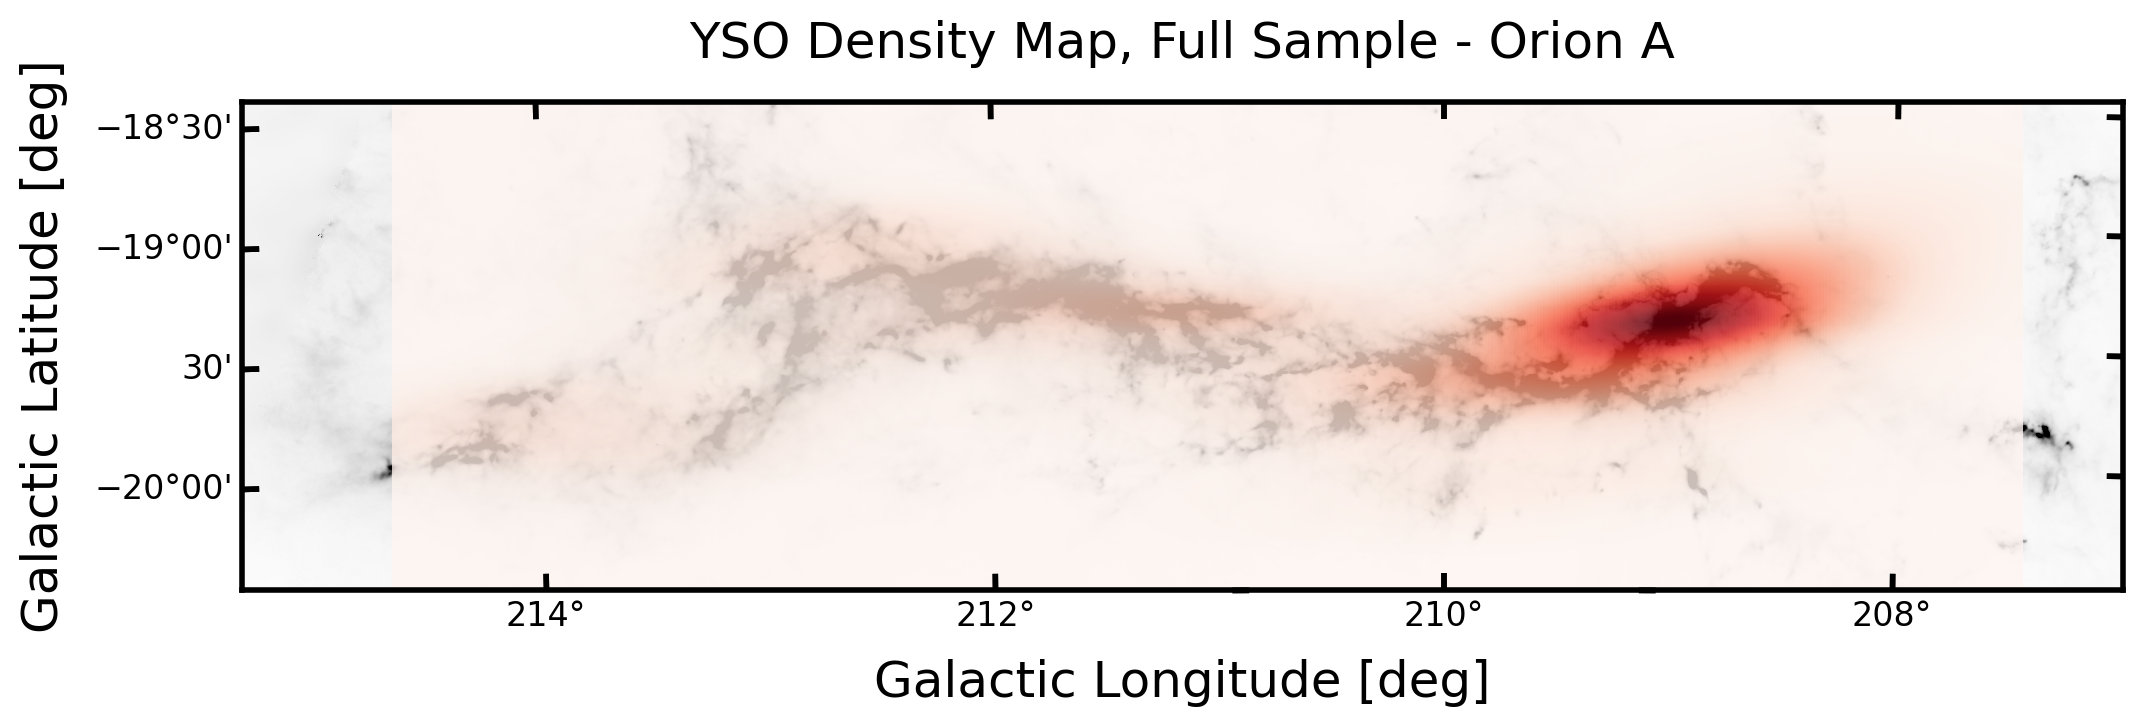
\includegraphics[width=0.75\textwidth]{figures/YSOs_density_Orion_A.png}
    \caption{YSO density map for Orion~A, overlaid on the column-density map. The coverage is limited by the extent of the YSO catalog, so some regions are not sampled.}
    \label{fig:YSOs_density_Map_A}
\end{figure}

\begin{figure}[h]
    \centering
    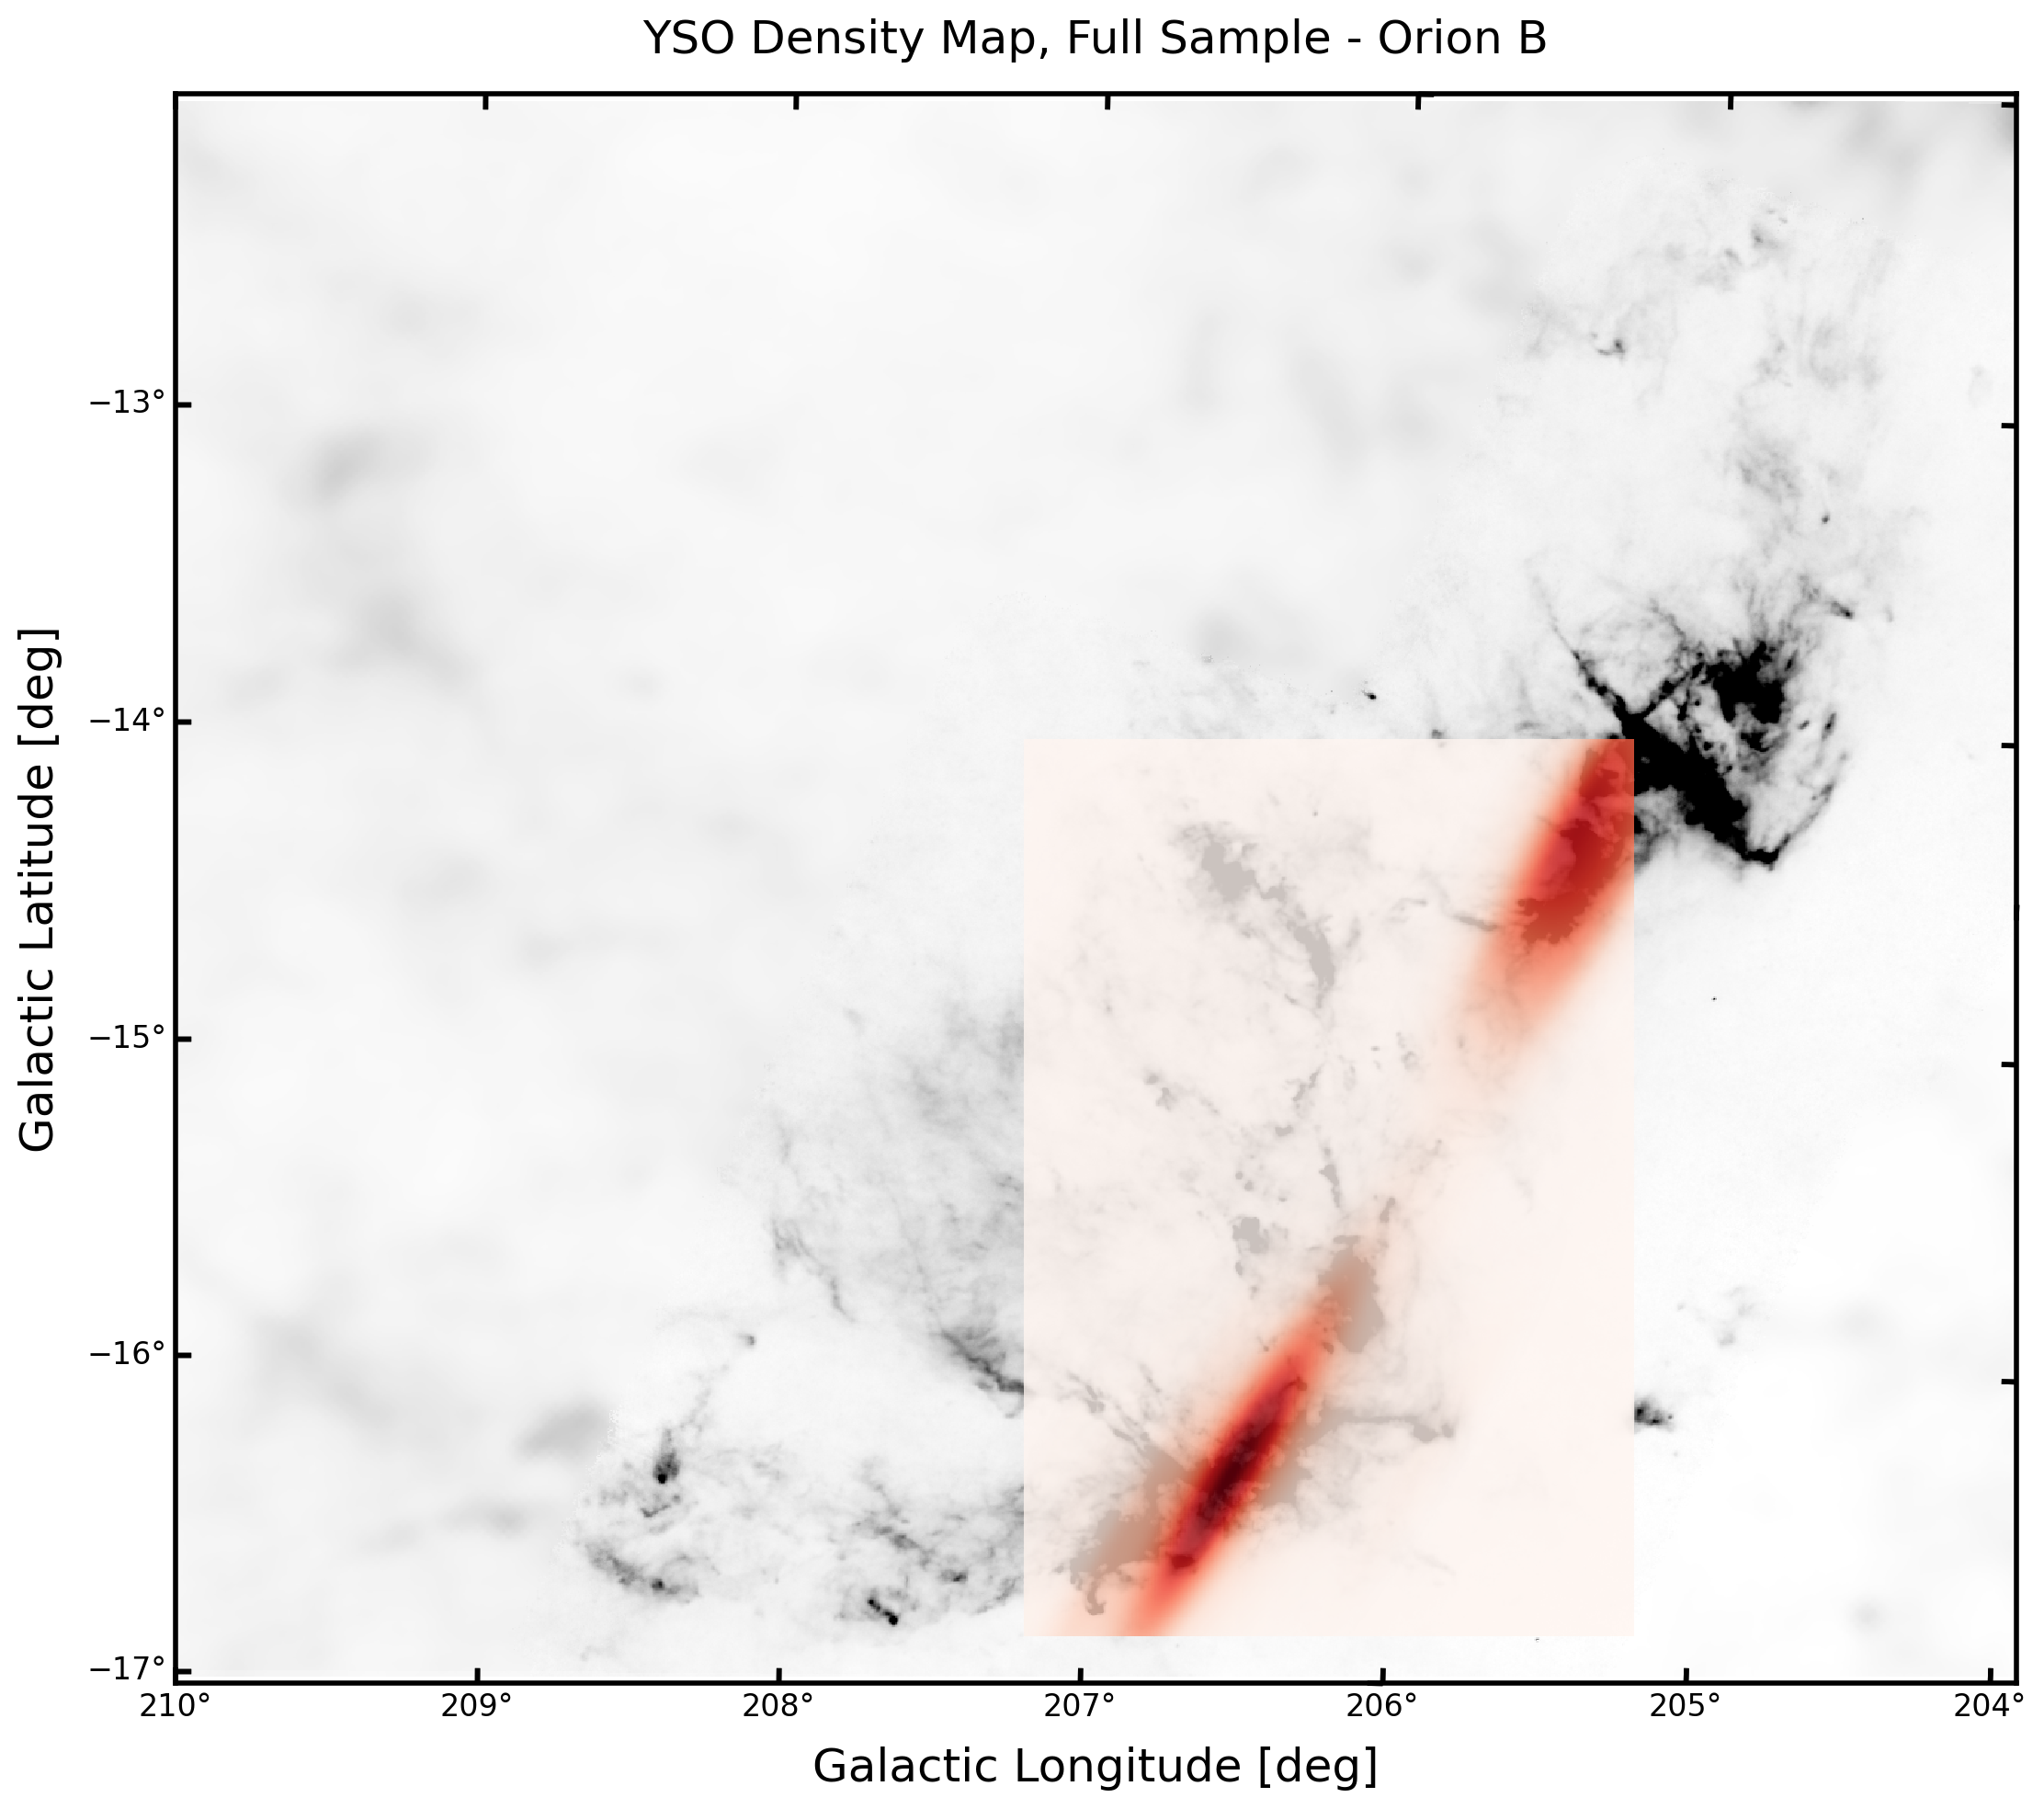
\includegraphics[width=0.5\textwidth]{figures/YSOs_density_Orion_B.png}
    \caption{YSO density map for Orion~A, overlaid on the column-density map. The coverage is limited by the extent of the YSO catalog, so some regions are not sampled.}
    \label{fig:YSOs_density_Map_B}
\end{figure}

\section{Simulations}

This section of the appendix provides more context to the results of the simulations and calculation of the uncertainties.

\subsection{Global Fractal Dimension}
% simulations global fractal dimension: D = 1 for simple shapes, gets higher the more complex it becomes 
% simulations global fractal dimension: GRF (scale free vs with scale) example
% simulations global fractal dimension: resolution effects

\subsection{Local Fractal Dimension}
% simulations local fractal dimension: resolution effects

\subsection{Euler Characteristic}

\subsection{Uncertainties}

\begin{figure}[h]
    \centering
    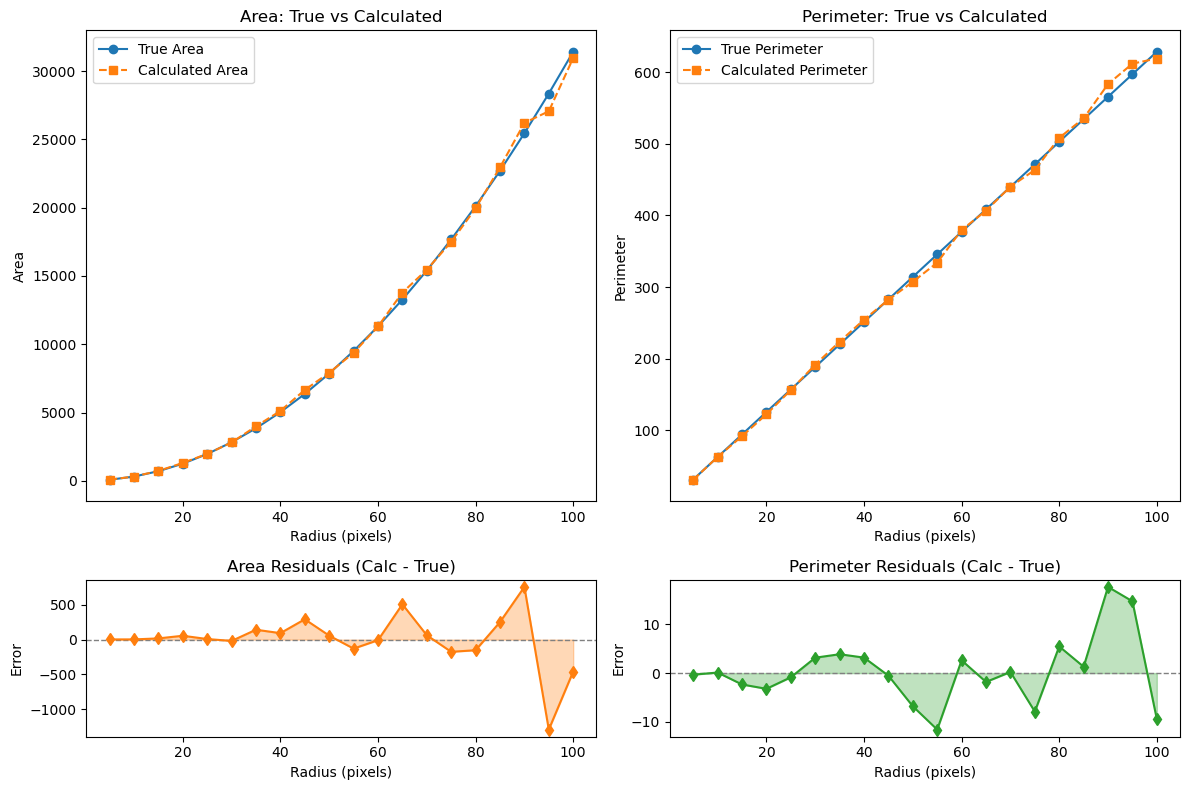
\includegraphics[width=0.75\textwidth]{figures/perimeter_area_uncertainties.png}
    \caption{Example of the uncertainty distributions in the measurements of perimeter and area from simulated structures (arbitrary units).}
    \label{fig:uncertainties}
\end{figure}

	
	
	
\end{document}